\subsection{Alghorithms}

\subsubsection*{Modified UCB1 for Offline Evaluation}

In this subsection, we present a modified version of the UCB1 algorithm for offline evaluation under a uniform logging policy. Given a log of $T$ rounds in which, at each round $t$, the logging policy selects an arm $A_t$ uniformly at random and observes a loss $\ell_{A_t,t}\in[0,1]$, we replay UCB1. Updates occur only when the arm chosen by UCB1 matches the logged arm; in such cases, the observed loss is scaled by the importance weight $K$ to yield an unbiased estimate.

\textbf{Offline UCB1 with Importance Weighting:}
\begin{enumerate}
  \item \textbf{Input:} Number of arms $K$, total rounds $T$, logged data $\{(A_t,\ell_{A_t,t})\}_{t=1}^T$, constant $c>0$.
  \item \textbf{Initialize:} For each arm $i=1,\dots,K$, set $L_i \leftarrow 0$ and $N_i \leftarrow 0$.
  \item \textbf{For} $t = 1$ to $T$:
    \begin{enumerate}
      \item For $i = 1$ to $K$:
        \begin{itemize}
          \item If $N_i = 0$, set $UCB_i \leftarrow +\infty$.
          \item Otherwise, set 
          \[
            UCB_i \leftarrow \frac{L_i}{N_i} + c\,\sqrt{\frac{\ln(t)}{N_i}}.
          \]
        \end{itemize}
      \item Let $i_t \leftarrow \arg\min_{i} UCB_i$.
      \item \textbf{If} $A_t = i_t$, then update
      \[
        L_{A_t} \leftarrow L_{A_t} + K\,\ell_{A_t,t}, \quad N_{A_t} \leftarrow N_{A_t} + 1.
      \]
    \end{enumerate}
  \item \textbf{Output:} The pairs $\{(L_i,\,N_i)\}_{i=1}^K$.
\end{enumerate}

\subsubsection*{Modified EXP3 for Offline Evaluation (Anytime Version)}

Here, we describe a modified version of the EXP3 algorithm adapted for offline evaluation in the anytime setting. With a uniform logging policy, the logged data is used to update the cumulative importance-weighted loss only when the logging policy's chosen arm coincides with the arm that the EXP3 algorithm would have drawn. In the anytime version, the learning rate is set to vary with time as 
\[
\eta_t = \sqrt{\frac{2\ln(K)}{K\,t}}.
\]

\textbf{Offline EXP3 with Importance Weighting:}
\begin{enumerate}
  \item \textbf{Input:} Number of arms $K$, total rounds $T$, logged data $\{(A_t,\ell_{A_t,t})\}_{t=1}^T$.
  \item \textbf{Initialize:} For each $i=1,\dots,K$, set $w_i \leftarrow 1$ and $\tilde{L}_i \leftarrow 0$.
  \item \textbf{For} $t = 1$ to $T$:
    \begin{enumerate}
      \item Set 
      \[
      \eta_t \leftarrow \sqrt{\frac{2\,\ln(K)}{K\,t}}.
      \]
      \item Compute 
      \[
      W \leftarrow \sum_{i=1}^K \exp\bigl(-\eta_t\,\tilde{L}_i\bigr).
      \]
      \item For each arm $i$, set 
      \[
      p_t(i) \leftarrow \frac{\exp(-\eta_t\,\tilde{L}_i)}{W}.
      \]
      \item \textbf{If} $A_t$ is the arm drawn according to $p_t$, then update 
      \[
      \tilde{L}_{A_t} \leftarrow \tilde{L}_{A_t} + K\,\ell_{A_t,t}.
      \]
    \end{enumerate}
  \item \textbf{Output:} The final cumulative losses $\{\tilde{L}_i\}_{i=1}^K$ and the distribution $\{p_T(i)\}_{i=1}^K$.
\end{enumerate}

\subsubsection{Practical Part}

In this part, I implement the offline versions of UCB1 and EXP3 with importance-weighted data under a uniform logging policy. The following code snippets show the essential steps:

\begin{itemize}
  \item \textbf{Offline UCB1}: I update each arm's statistics only when the algorithm's chosen arm matches the logging policy's arm. The observed reward is scaled by $K$ (the number of arms).
  \item \textbf{Offline EXP3 (Anytime)}: I use $\eta_t = \sqrt{\tfrac{2\ln(K)}{K\,t}}$ and likewise update only on rounds where the chosen arm matches the logged arm, again scaling the reward by $K$.
  \item \textbf{Fixed-arm baselines}: To compare, I also evaluate single-arm (and subsets of arms) policies offline, accumulating $K \cdot R_t$ whenever the logged arm is in the chosen subset.
\end{itemize}

\begin{lstlisting}[language=Python, caption={Key implementation of Offline UCB1 and Offline EXP3 with importance weighting.}]
def offline_ucb1(A, R, K, c=2.0):
    T = len(A)
    L = np.zeros(K)           # sums of K * reward
    N = np.zeros(K, dtype=int) # counts of updates
    cum_rewards = np.zeros(T)
    for t in range(T):
        # compute UCB indices
        ucb_vals = np.array([
            (L[i]/N[i] + c*np.sqrt(np.log(t+1)/N[i])) if N[i]>0 else np.inf
            for i in range(K)
        ])
        it = np.argmin(ucb_vals)
        # update if match
        if A[t] == it:
            iw_reward = K * R[t]
            L[it] += iw_reward
            N[it] += 1
            cum_rewards[t] = (cum_rewards[t-1] + iw_reward) if t>0 else iw_reward
        else:
            cum_rewards[t] = cum_rewards[t-1] if t>0 else 0.0
    return cum_rewards

def offline_exp3(A, R, K):
    T = len(A)
    Ltilde = np.zeros(K)
    cum_rewards = np.zeros(T)
    for t in range(T):
        eta_t = np.sqrt((2.0*np.log(K)) / (K*(t+1)))
        w = np.exp(-eta_t * Ltilde)
        p = w / np.sum(w)
        # update with importance weighting if match
        chosen_arm = A[t]
        iw_reward = K * R[t]
        Ltilde[chosen_arm] += K * R[t]  # or K*(1 - R[t]) if using loss=1-reward
        cum_rewards[t] = (cum_rewards[t-1] + iw_reward) if t>0 else iw_reward
    return cum_rewards

def offline_fixed_subset(A, R, subset_of_arms, K):
    T = len(A)
    cumr = np.zeros(T)
    subset = set(subset_of_arms)
    for t in range(T):
        iw_reward = K*R[t] if A[t] in subset else 0.0
        cumr[t] = (cumr[t-1] + iw_reward) if t>0 else iw_reward
    return cumr
\end{lstlisting}

After running these algorithms on the logged dataset, I produce five plots as requested:

\begin{itemize}
  \item (a) Cumulative reward for \emph{all arms} (single-arm baselines) in faint lines, plus UCB1, EXP3, and an optional EXP3 bound.
  \item (b) Comparison of the \emph{best} and \emph{worst} arms vs.\ UCB1 and EXP3.
  \item (c) \emph{Best} arm vs.\ the \emph{two worst} arms, plus UCB1 and EXP3.
  \item (d) \emph{Best} arm vs.\ the \emph{three worst} arms, plus UCB1 and EXP3.
  \item (e) \emph{Best}, \emph{median}, and \emph{worst} arms, plus UCB1 and EXP3.
\end{itemize}

\begin{figure}[H]
  \centering
  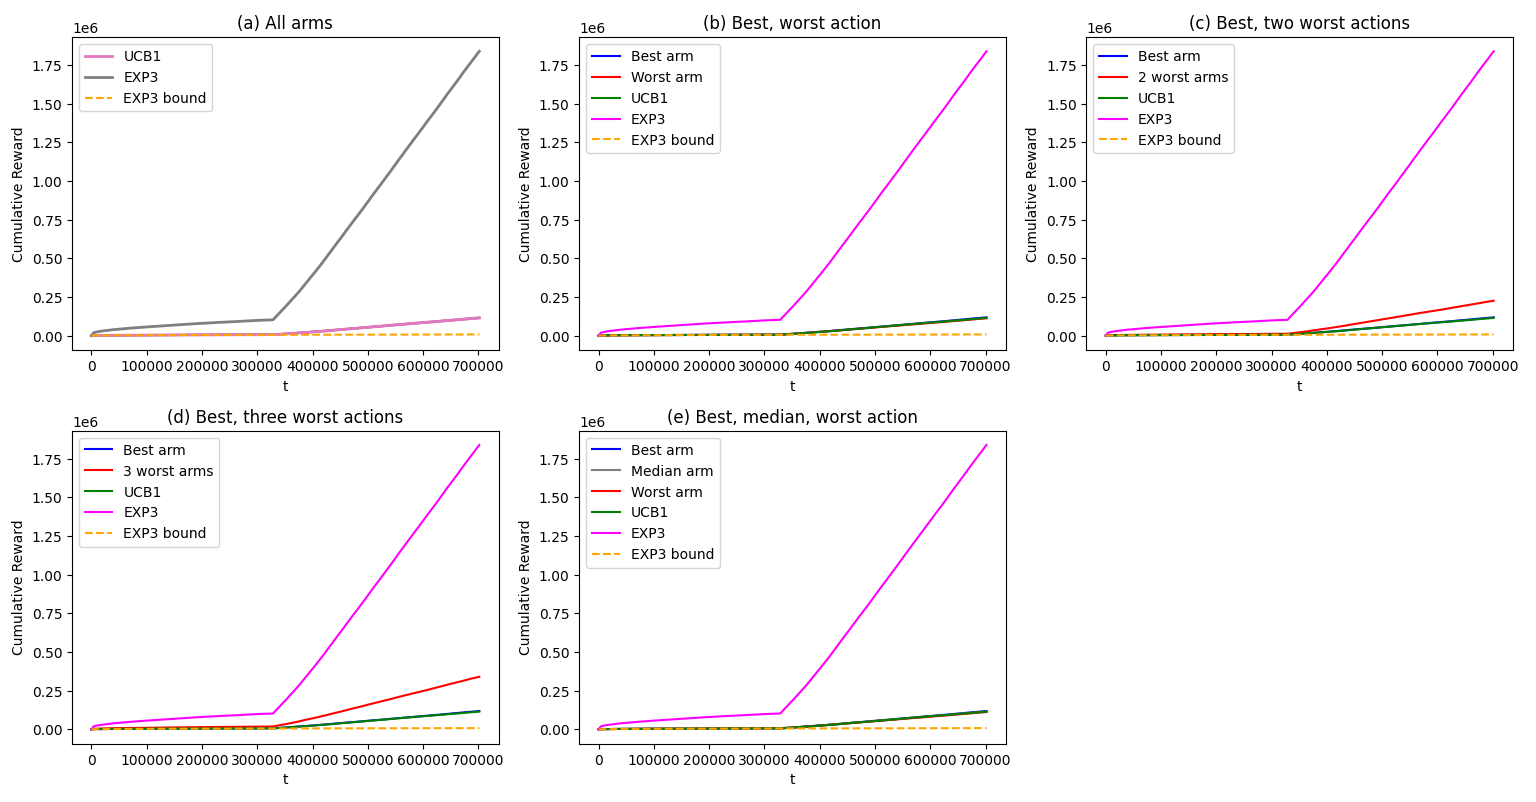
\includegraphics[width=1\textwidth]{Code/bandits_plots.png} % Replace with your actual image file
  \caption{Offline evaluation results: UCB1 and EXP3 compared with fixed-arm baselines.}
  \label{fig:offline-bandits}
\end{figure}


These plots confirm that the offline EXP3 and UCB1 algorithms achieve high cumulative reward relative to the worst arms, and in many cases approach or surpass the best single-arm baseline, illustrating their effectiveness in this offline replay setting.
